\documentclass{article}

\usepackage{graphicx}
\usepackage{tikz}
\usepackage{tikzsymbols}
\usetikzlibrary{calc,patterns,shapes.geometric}
\pagestyle{empty}
\usepackage[margin=0pt]{geometry}
\geometry{papersize={14in,12in}}

\def\centerarc[#1](#2)(#3:#4:#5){\draw[#1] ($(#2)+({#5*cos(#3)},{#5*sin(#3)})$) arc (#3:#4:#5);}

\begin{document}
	\begin{figure}
		\centering
		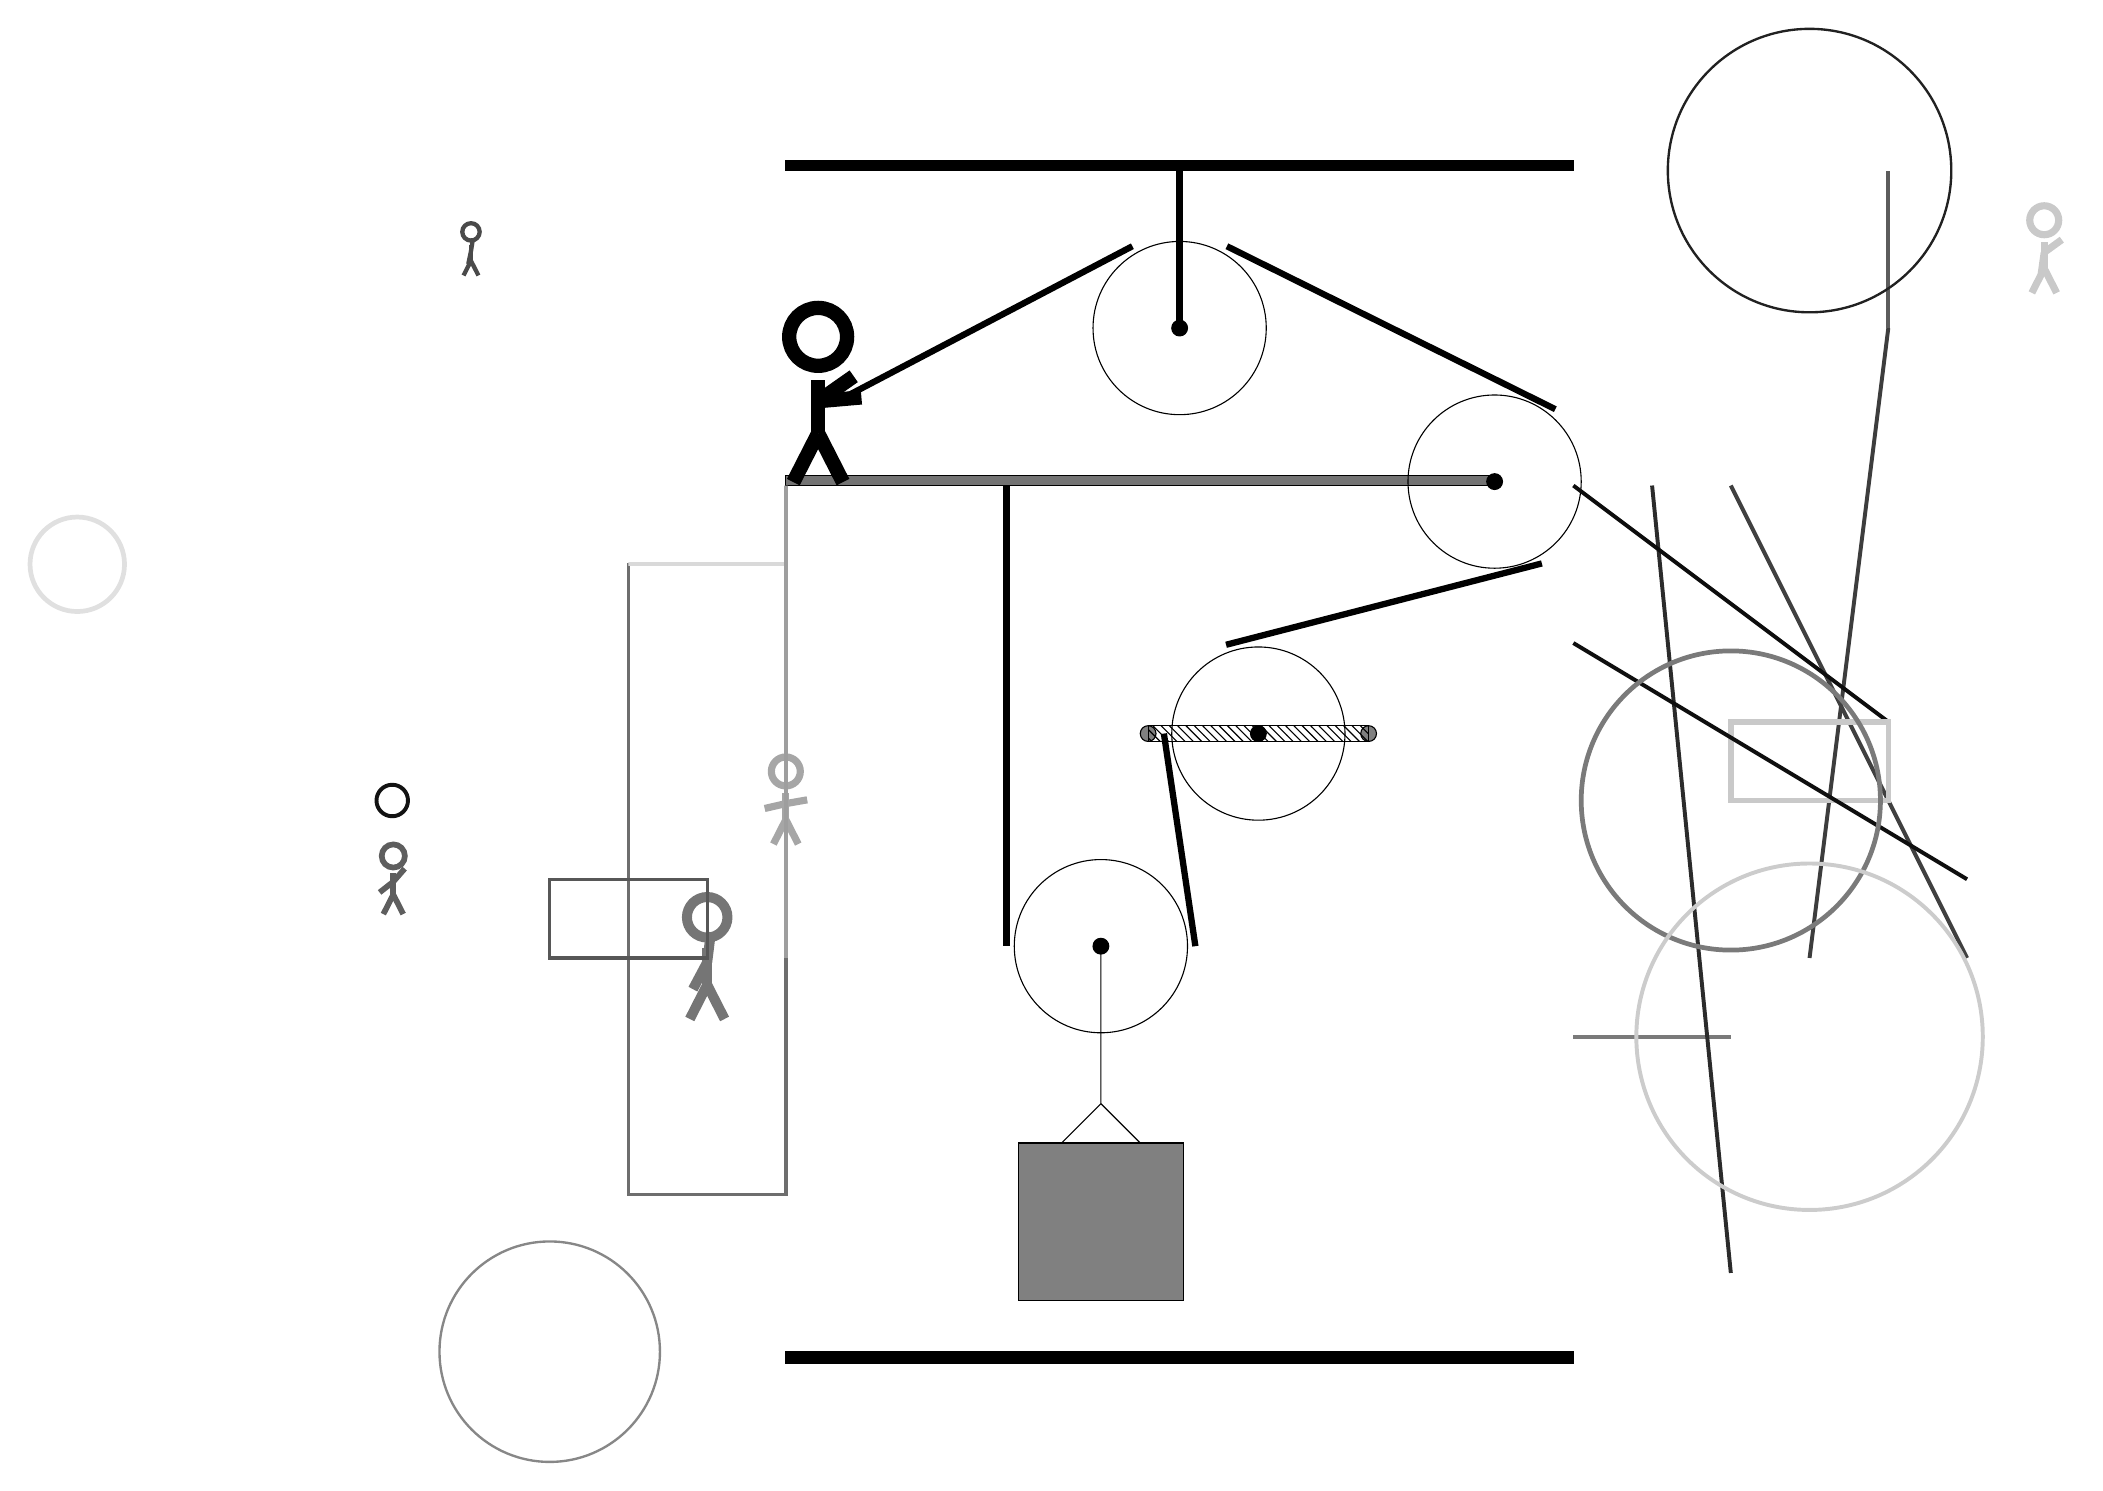
\begin{tikzpicture}
			%%%%% START %%%%%
			
			\draw[fill=black] (-2, 13) rectangle (8, 13.125);
			
			\draw[fill=black!55] (-2, 9) rectangle (7, 9.125);
			
			\draw (2, 3.15) circle (1.1);
			\draw[fill=black] (2, 3.15) circle (0.1);
			
			\draw (7, 9.05) circle (1.1);
			\draw[fill=black] (7, 9.05) circle (0.1);
			
			\draw[fill=white](4, 5.85) circle (1.1);
			\draw[fill=black] (4, 5.85) circle (0.1);
			\draw[fill=black!50] (2.6, 5.85) circle (0.1);
			\draw[fill=black!50] (5.4, 5.85) circle (0.1);
			\draw[pattern=north west lines, pattern color=black] (2.6, 5.95) rectangle (5.4, 5.75);
			
			\draw (3, 11) circle (1.1);
			\draw[fill=black] (3, 11) circle (0.1);
			\draw[line width=0.8mm] (3, 11) -- (3, 13);
			
			\draw[line width=0.4mm, color=black!57] (-2, 0) rectangle (-4, 8);
			
			\draw[line width=0.5mm, color=black!76](12, 11) -- (11, 3);
			\draw [line width=0.3mm, color=black!47](-5, -2) circle (1.4);
			\node[line width=0.7mm, color=black!63] at (-7, 4) {\Strichmaxerl[4][38][49]};
			\draw[line width=0.5mm, color=black!52](8, 2) -- (10, 2);
			\node[line width=0.4mm, color=black!71] at (-6, 12) {\Strichmaxerl[3][78][81]};
			\draw [line width=0.6mm, color=black!12](-11, 8) circle (0.6);
			\node[line width=0.2mm, color=black!54] at (-3, 3) {\Strichmaxerl[7][62][83]};
			\node[line width=0.6mm, color=black!35] at (-2, 5) {\Strichmaxerl[5][13][10]};
			\draw [line width=0.5mm, color=black!93](-7, 5) circle (0.2);
			\draw[line width=0.5mm, color=black!83](9, 9) -- (10, -1);
			\draw[line width=0.5mm, color=black!64](12, 11) -- (12, 13);
			\draw [line width=0.3mm, color=black!87](11, 13) circle (1.8);
			
			\draw[line width=0.5mm, color=black!75](13, 3) -- (10, 9);
			\draw[line width=0.4mm, color=black!66] (-3, 3) rectangle (-5, 4);
			\draw[line width=0.5mm, color=black!95](12, 6) -- (8, 9);
			\draw[line width=0.7mm, color=black!21] (10, 6) rectangle (12, 5);
			
			\draw[line width=0.5mm, color=black!94](13, 4) -- (8, 7);
			\draw [line width=0.6mm, color=black!52](10, 5) circle (1.9);
			\node[line width=0.7mm, color=black!21] at (14, 12) {\Strichmaxerl[5][82][36]};
			\draw[line width=0.5mm, color=black!15] (-4, 8) rectangle (-2, 8);
			
			\draw[line width=0.6mm, color=black!38] (-2, 3) rectangle (-2, 9);
			\draw [line width=0.5mm, color=black!20](11, 2) circle (2.2);
			
			\draw (2, 3.15) -- (2, 1.15) -- (1.5, 0.65) -- (2.5, 0.65) -- (2, 1.15);
			\draw[fill=black!50] (0.95, 0.65) rectangle (3.05, -1.35);
			
			\draw[line width=0.8mm] (0.8, 9) -- (0.8, 3.15);
			\centerarc[line width=0.8mm](2, 3.15)(180:360:1.2000000000000002);
			\draw[line width=0.8mm](3.2, 3.15) -- (2.8, 5.85);
			\centerarc[line width=0.8mm](4, 5.85)(110:180:1.2000000000000002);
			\draw[line width=0.8mm](3.5896, 6.9776) -- (7.6, 8.0108);
			\centerarc[line width=0.8mm](7, 9.05)(-60:50:1.2000000000000002);
			\draw[line width=0.8mm](7.7714, 9.9692) -- (3.6, 12.0392);
			\centerarc[line width=0.8mm](3, 11)(60:120:1.2000000000000002);
			\draw[line width=0.8mm](2.4, 12.0392) -- (-1.2, 10.15);
			
			\node at (-1.5, 10.15) {\Strichmaxerl[10][-175][35]};
			
			\draw[fill=black] (-2, -2) rectangle (8, -2.15);
			
			%%%%% END %%%%%
		\end{tikzpicture}
	\end{figure}	
\end{document}